

In this chapter, PROM performance in modeling a multi-element rocket combustor experiencing high-frequency combustion instability is examined. This model is based on experiments conducted with the nine-element Transverse Instability Combustor Purdue University by Orth \textit{et al.}~\cite{Orth2018}. In the following section, only a simplified description of the experiment as it pertains to the numerical model is described; the reader is encouraged to find greater detail on the experiment's design in~\cite{Orth2018}. As with the CVRC, this test article was designed in tandem with CFD researchers in an effort to establish a rocket combustor benchmark for the development of advanced reacting flow LES solvers. In this case, the number of parallel propellant injectors is increased to nine, introducing additional complexity due to interactions between injectors in the presence of strong transverse combustion instabilities. Indeed, work by Harvazinski \textit{et al.}~\cite{Harvazinski2019} was able to reasonably replicate the experimental self-excited combustion instability via LES with a reduced finite-rate chemistry mechanism. However, as will be demonstrated shortly, the computational cost of such simulations is exceptionally high and precludes any usefulness in the engineering design process. As such, this case provides an excellent target for reduced-order modeling.

\subsection{Full-order Model}
%
The computational model presented here derives from the work by Harvazinski \textit{et al.}~\cite{Harvazinski2019}, using the same computational mesh, but marginally different boundary conditions and a different reaction mechanism. The spatial domain does not include the oxidizer preburner, oxidizer manifold, or fuel manifold elements of the experimental test article. A cutaway of the spatial domain is shown in Fig.~\ref{fig:nineElemGeomXY}, and an isometric view of the combustor is shown in Fig.~\ref{fig:nineElemGeomIso}. The combustor is composed of a linear array of nine coaxial propellant injection elements, each spaced centerline-to-centerline by 26.67 mm apart. The oxidizer posts extend 96.01 mm upstream of the dump plane, and has a diameter of 11.25 mm upstream of the fuel injection port. Each oxidizer post supplies 96.5\% gaseous oxygen and 3.5\% water vapor (by weight) at 636 K. The entire oxidizer injection assembly supplies oxidizer at a rate of 0.7575 kg/s. Fuel is supplied by radial injection approximately 42 mm upstream of the dump plane, after which flow is turned 90$^{\circ}$ to exit the annular fuel port and mix with the oxidizer approximately 11.34 mm upstream of the dump plane. The inner diameter of each fuel annulus measures 13 mm, and the outer diameter (also the diameter of the propellant injection port into the combustion chamber) measures 15.75 mm. Each fuel injector supplies 100\% gaseous methane at 287.6 K at a rate of 0.02369 kg/s. The main combustion chamber (upstream of the nozzle) measures 118.5 mm long ($x$-direction), 240 mm wide ($y$-direction), and 30.5 mm deep ($z$-direction). The nozzle is 81.5 mm long, and terminates in an exit port 142.1 mm wide and 10.8 mm deep.

\begin{sidewaysfigure}
	\begin{minipage}{0.49\linewidth}
		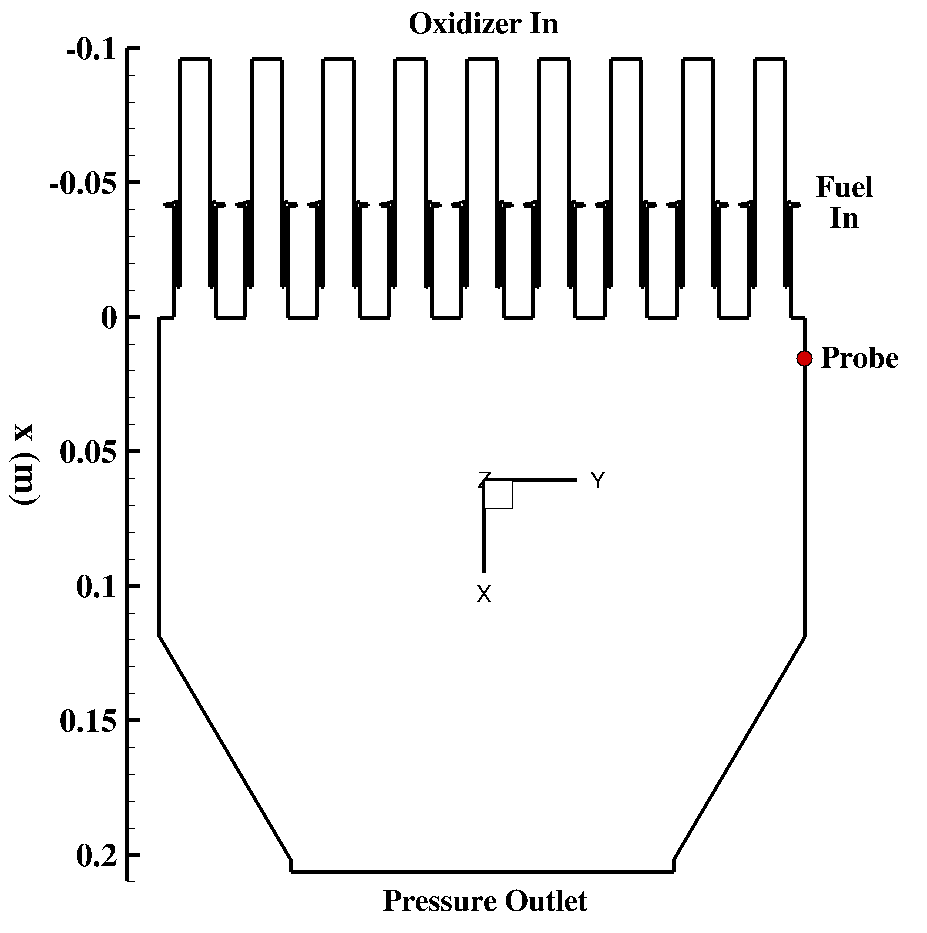
\includegraphics[width=0.99\linewidth]{Chapters/HPROMResults/Images/nineElem/geom_xy.png}
		\caption{\label{fig:nineElemGeomXY}Nine-element combustor geometry, $x-y$ cutaway.}
	\end{minipage}
	\begin{minipage}{0.49\linewidth}
		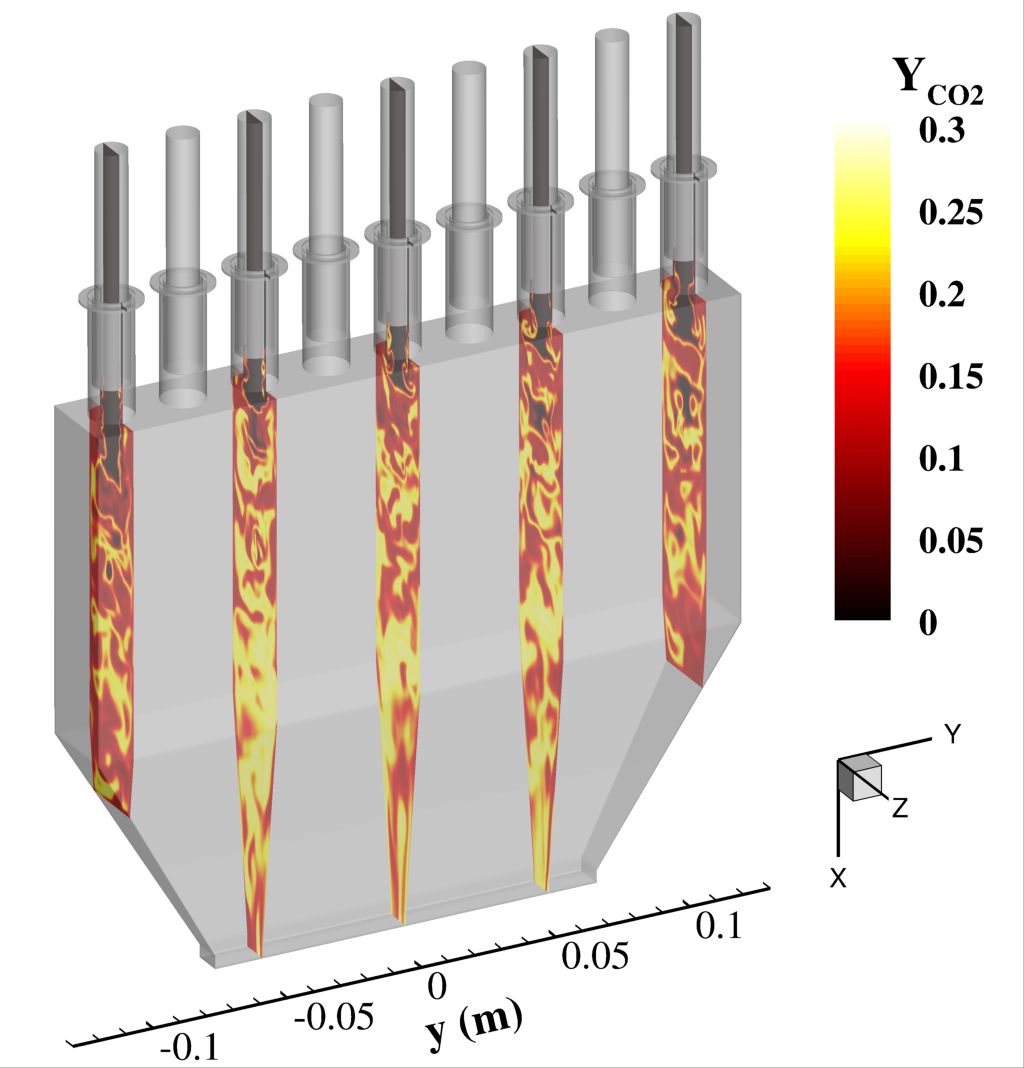
\includegraphics[width=0.99\linewidth]{Chapters/HPROMResults/Images/nineElem/geom_iso.png}
		\caption{\label{fig:nineElemGeomIso}Nine-element combustor geometry, isometric view, with $Y_{\text{CO}_2}$ $y-z$ slices at $\timeVar = 21.5$ ms.}
	\end{minipage}
\end{sidewaysfigure}

Mass flow rate boundary conditions are applied to the oxidizer and fuel inlets, though a single rate is enforced for the entire oxidizer inlet area, while individual rates are enforced for each fuel inlet. Adiabatic, no-slip wall conditions are enforced at all walls. A fixed pressure outlet is enforced at the nozzle exit, specifying an exit pressure of 101,325 Pa to model venting to atmosphere.

Reactions are modeled by a 12-species (plus inert nitrogen), 38-reaction finite-rate mechanism referred to as FFCMy-12, which is developed by Xu and Wang~\cite{Wang2018,Xu2018} as a reduced mechanism of the larger FFCM-1 mechanism~\cite{ffcm1} tailored for combustion of methane and oxygen in rocket combustors. As mentioned in Section~\ref{sec:finiterate}, this mechanism includes third-body low-pressure corrections of the Hinshelwood~\cite{Hinshelwood1926} and Troe~\cite{Gilbert1983} forms. This mechanism has been utilized previously in the simulation of traditional liquid rocket engines~\cite{Harvazinski2020,Harvazinski2021} as well as rotating detonation engines~\cite{Prakash2021,Batista2021}. The fluid is treated as a thermally-perfect gas, and thermodynamic and transport properties are computed by the empirical fit models described in Section~\ref{subsec:gasModels}. Subgrid dissipation is modeled via the Nicoud $\sigma$-model described in Section~\ref{subsec:subgrid}.

The computational mesh is composed of 14,387,292 hexahedral cells, resulting in a total full-order dimension of $\numDOF = 244,583,964$. To the best of the author's knowledge, this represents the largest case examined for PROMs of unsteady fluid flows, and also accounts for a significant increase in modeling complexity relative to comparable studies of aerodynamics problems.

The FOM is initialized as follows. The entire domain is initialized with zero velocity and 1.138 MPa pressure. The oxidizer posts and propellant injection ports (excluding the fuel annuli) are initialized with 96.5\% oxygen and 3.5\% water vapor at 636 K. The fuel annuli are initialized with 100\% methane at 287.6 K. The combustion chamber is initialized with hot products (44\% water vapor and 56\% carbon dioxide) at 2,000 K. The physical time step size is $\dt = 0.1 \mu$s, and the FOM is first run for 215,000 steps (21.5 ms) to allow the transverse instability to initiate and for the flow to become statistically stationary. The instability is visualized in Fig.~\ref{fig:nineElemFOMPressure}, where a high-pressure wave traverses the width of the combustion chamber (reflecting from the walls) over the course of approximately 0.195 ms. The pressure wave is accompanied by heightened local heat release, which can be seen in Fig.~\ref{fig:nineElemFOMHeat}.

\begin{figure}
	\begin{minipage}{0.49\linewidth}
		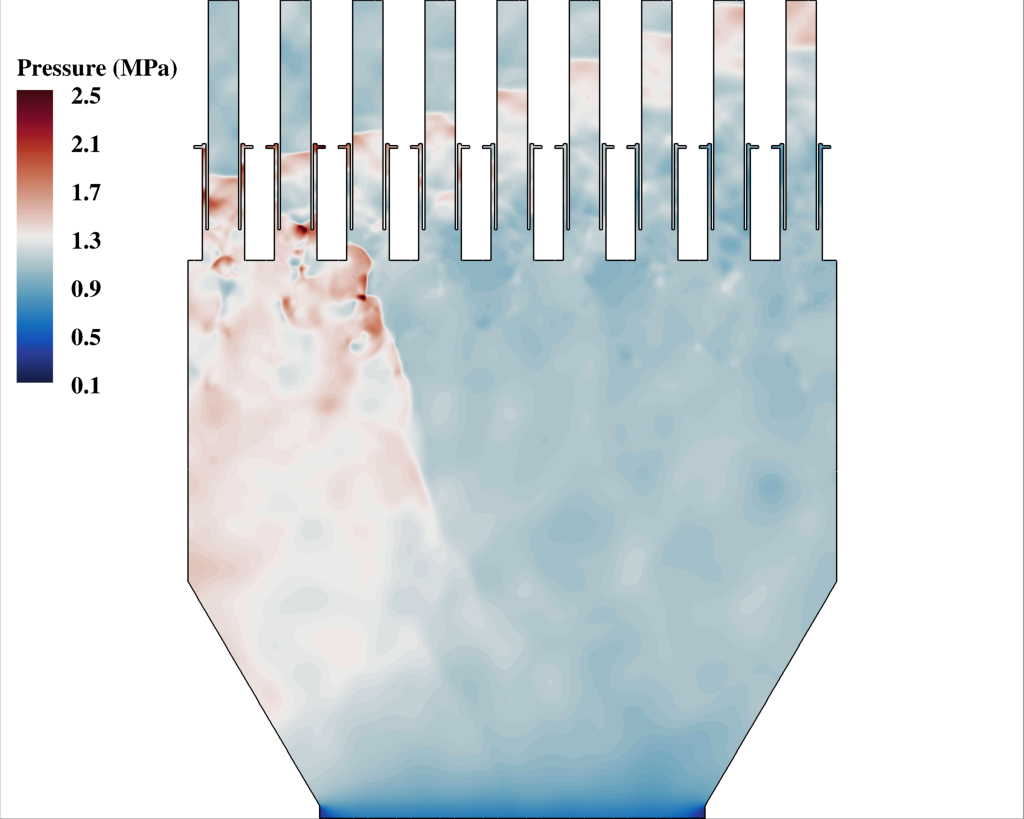
\includegraphics[width=0.99\linewidth,trim={0.5em 0em 6cm 0em},clip]{Chapters/HPROMResults/Images/nineElem/example_snaps/example_pressure_z.png}
	\end{minipage}
	\begin{minipage}{0.49\linewidth}
		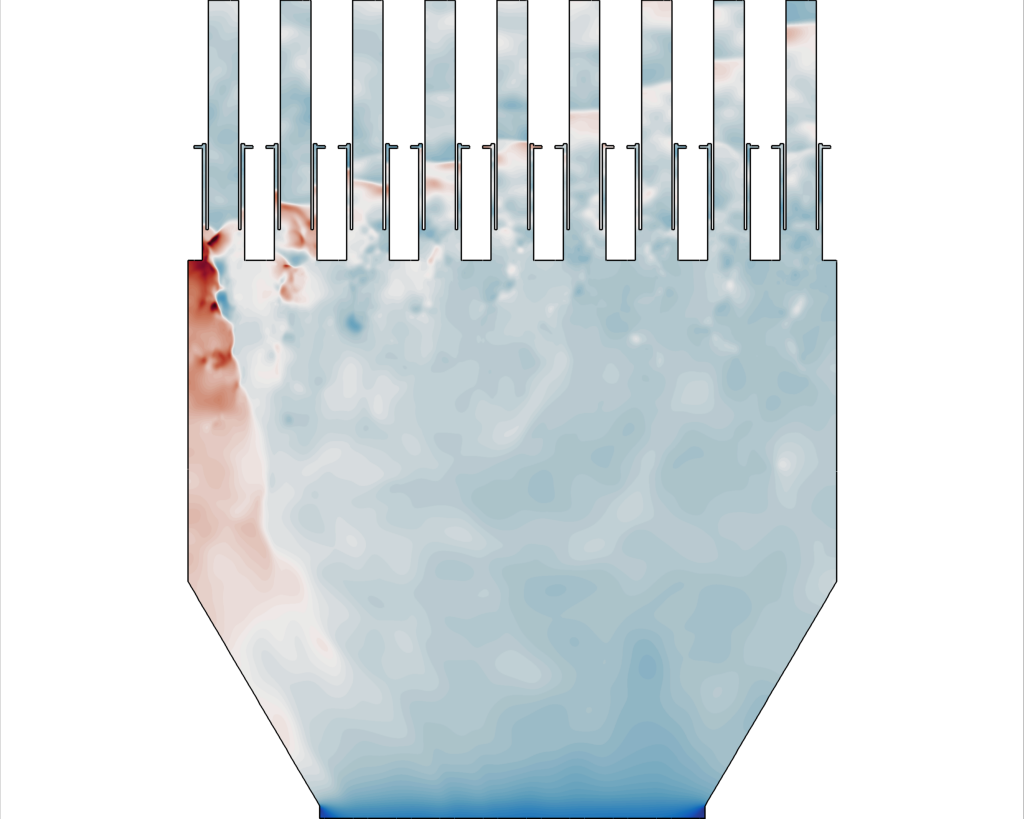
\includegraphics[width=0.99\linewidth,trim={6cm 0em 0.5em 0em},clip]{Chapters/HPROMResults/Images/nineElem/example_snaps/example_pressure_z_216000.png}
	\end{minipage}

	\begin{minipage}{0.49\linewidth}
		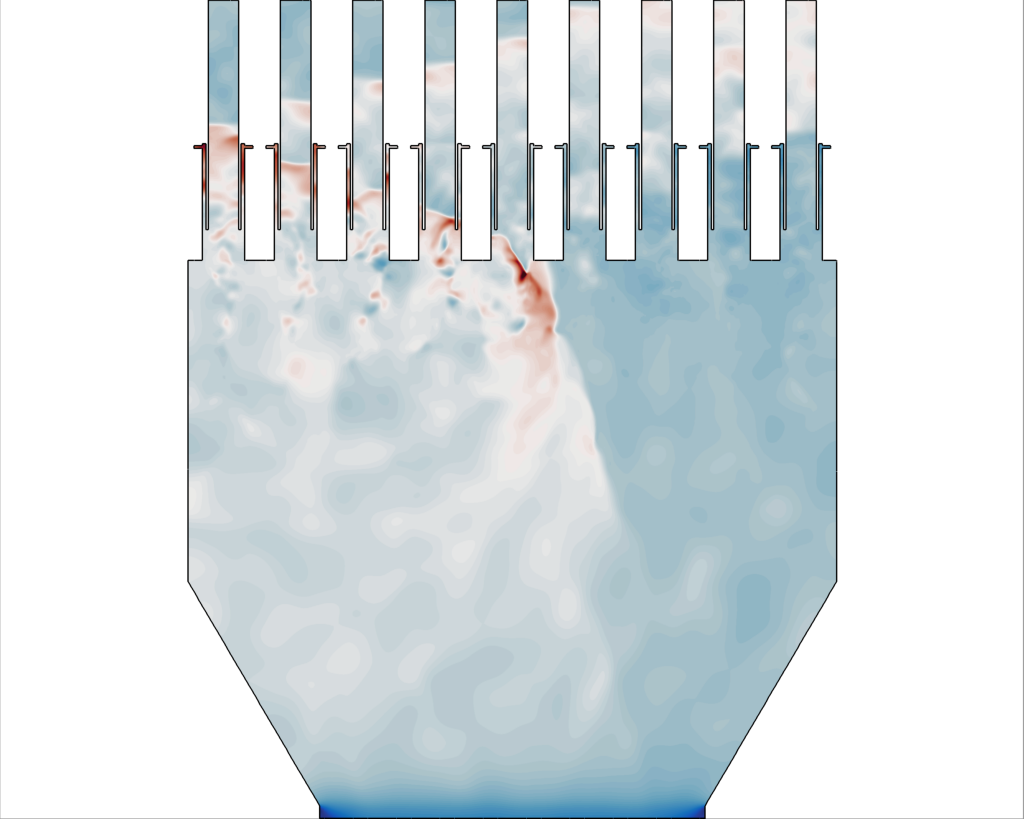
\includegraphics[width=0.99\linewidth,trim={0.5em 0em 6cm 0em},clip]{Chapters/HPROMResults/Images/nineElem/example_snaps/example_pressure_z_217000.png}
	\end{minipage}
	\begin{minipage}{0.49\linewidth}
		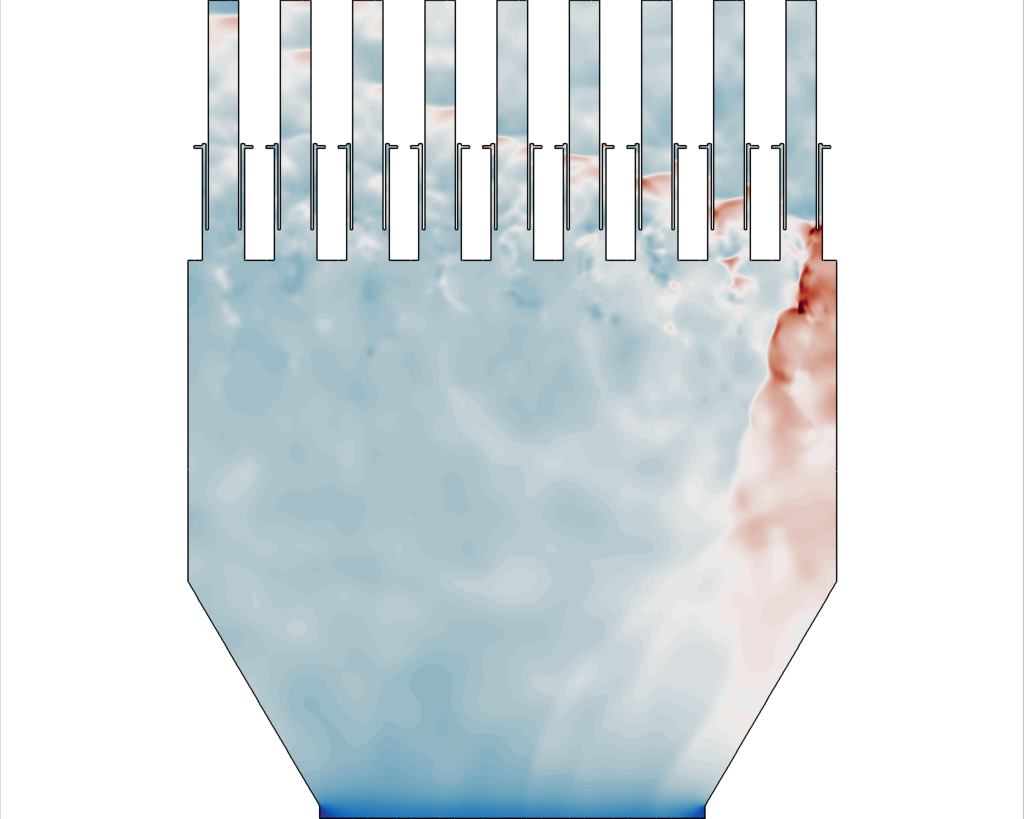
\includegraphics[width=0.99\linewidth,trim={6cm 0em 0.5em 0em},clip]{Chapters/HPROMResults/Images/nineElem/example_snaps/example_pressure_z_218000.png}
	\end{minipage}
	\caption{\label{fig:nineElemFOMPressure}FOM pressure contours for $x-y$ plane slice at $\timeVar = $ 21.5 (top left), 21.6 (top right), 21.7 (bottom left) and 21.8 (bottom right) ms.}
\end{figure}

\begin{figure}
	\begin{minipage}{0.49\linewidth}
		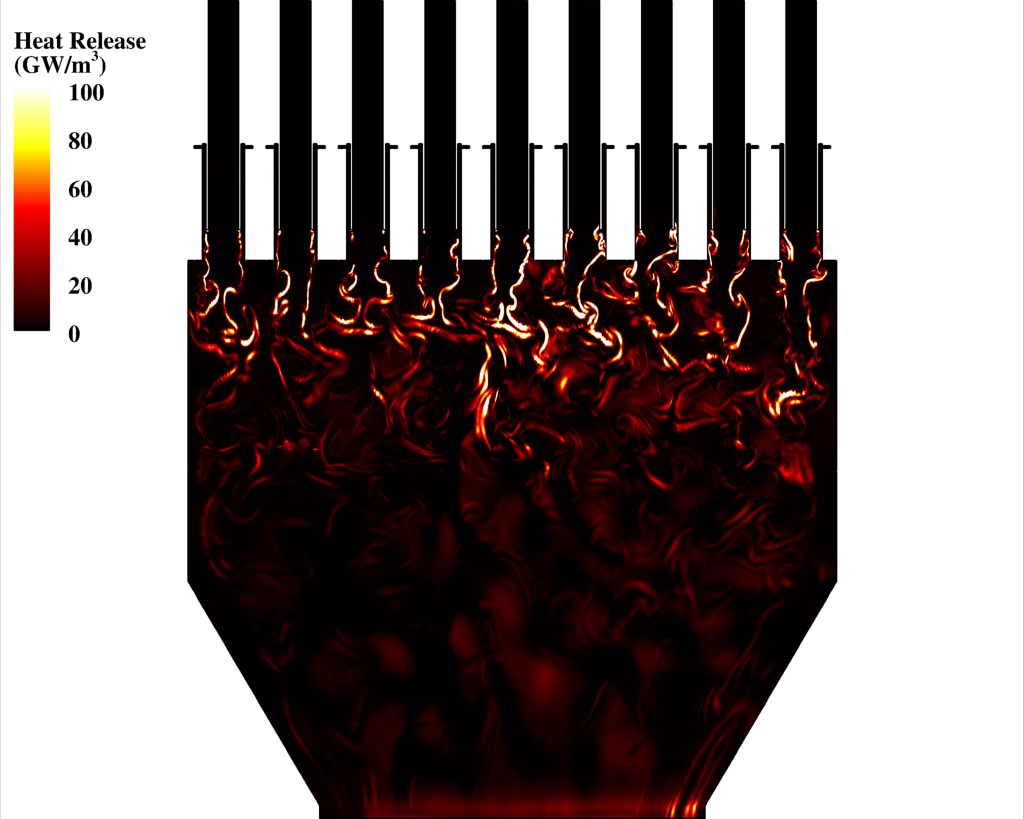
\includegraphics[width=0.99\linewidth,trim={0.5em 0em 6cm 0em},clip]{Chapters/HPROMResults/Images/nineElem/example_snaps/example_heat_z.png}
	\end{minipage}
	\begin{minipage}{0.49\linewidth}
		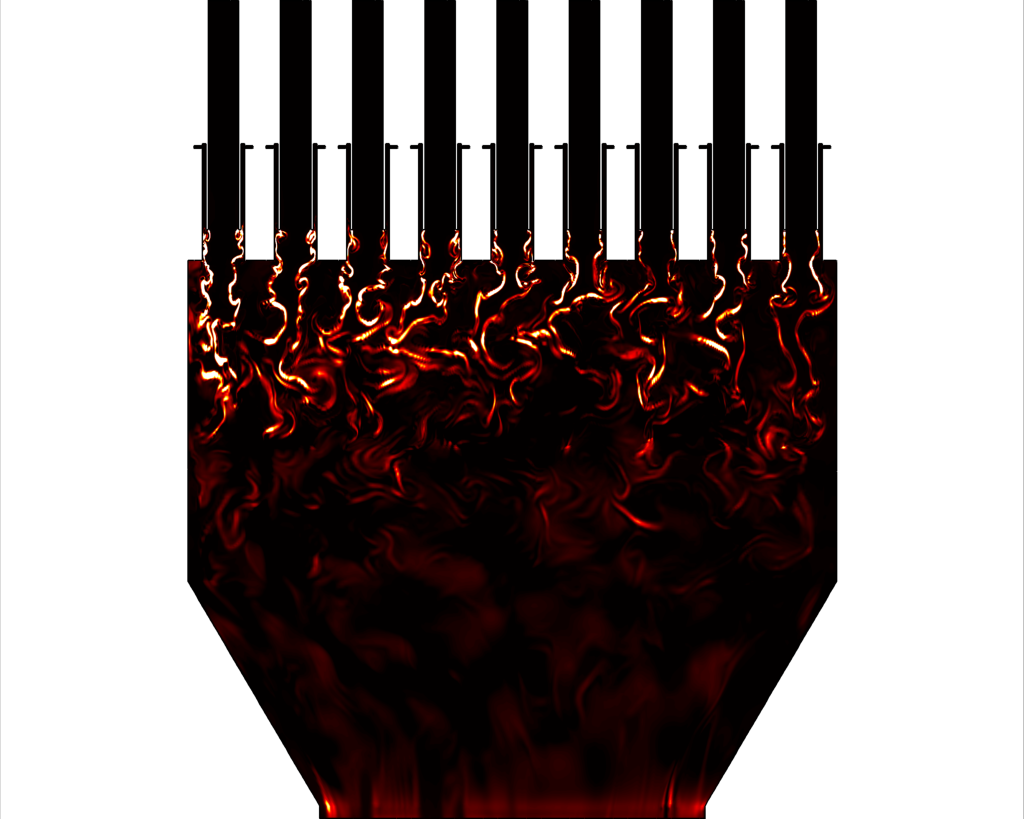
\includegraphics[width=0.99\linewidth,trim={6cm 0em 0.5em 0em},clip]{Chapters/HPROMResults/Images/nineElem/example_snaps/example_heat_z_216000.png}
	\end{minipage}

	\begin{minipage}{0.49\linewidth}
		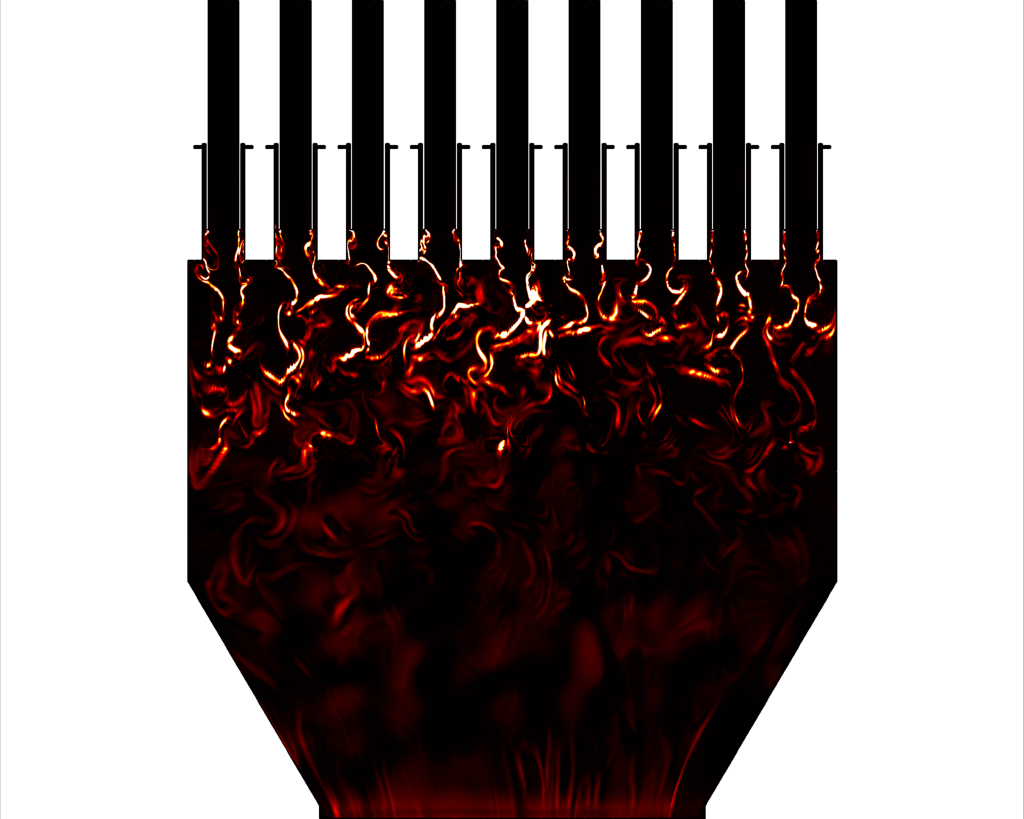
\includegraphics[width=0.99\linewidth,trim={0.5em 0em 6cm 0em},clip]{Chapters/HPROMResults/Images/nineElem/example_snaps/example_heat_z_217000.png}
	\end{minipage}
	\begin{minipage}{0.49\linewidth}
		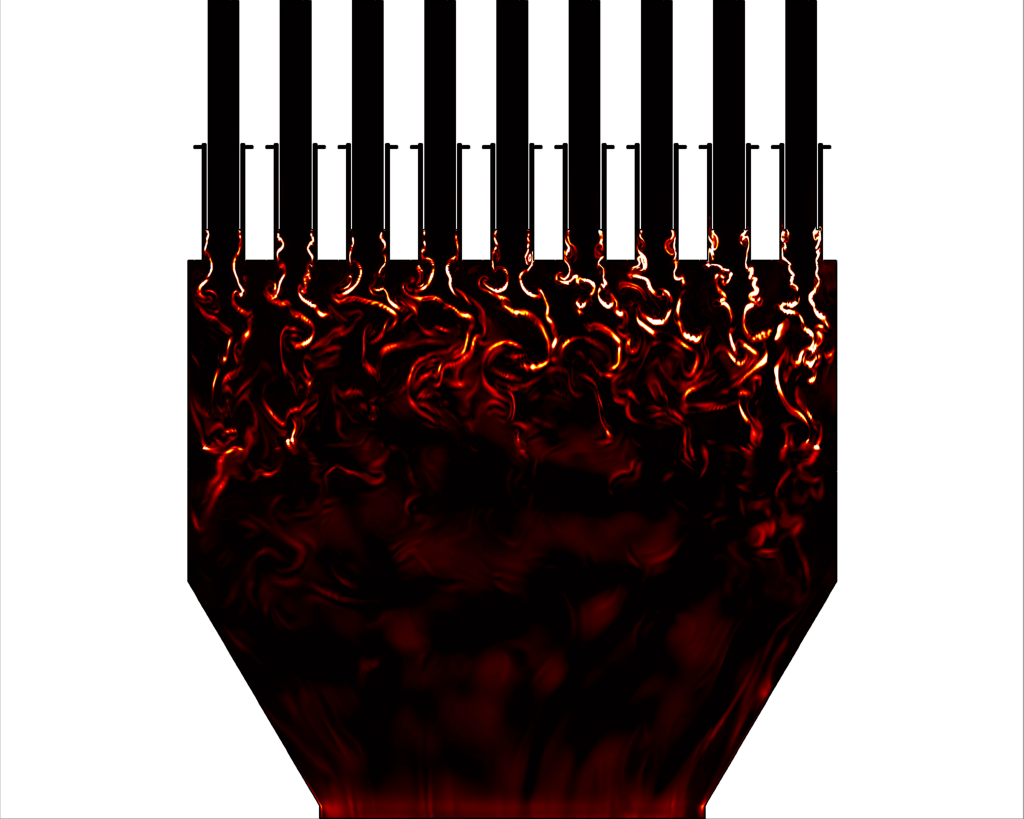
\includegraphics[width=0.99\linewidth,trim={6cm 0em 0.5em 0em},clip]{Chapters/HPROMResults/Images/nineElem/example_snaps/example_heat_z_218000.png}
	\end{minipage}
	\caption{\label{fig:nineElemFOMHeat}FOM heat release contours for $x-y$ plane slice at $\timeVar = $ 21.5 (top left), 21.6 (top right), 21.7 (bottom left) and 21.8 (bottom right) ms.}
\end{figure}

Starting at $\timeVar = 21.5$ ms, snapshots of the primitive and conservative states are collected at every time step until $\timeVar = 21.89$, resulting in 3,901 snapshots (including $\stateVec(\timeVar = 21.5 \text{ms})$). The POD residual energy decay is shown in Fig.~\ref{fig:nineElemPODEnergy}. Achieving 1\%, 0.1\%, and 0.01\% of the conservative state POD residual energy requires 79, 177, and 300 modes respectively. For the primitive state, this requires 67, 144, and 262 modes respectively. As with the truncated CVRC, this case exhibits an extremely slow POD residual energy decay characteristic of such a highly-nonlinear convection-dominated flow. The projection error of the primitive and conservative state datasets are shown in Figs.~\ref{fig:nineElemProjErrPrim} and~\ref{fig:nineElemProjErrCons} respectively. Interestingly, again the transverse and depth-wise velocity represent the largest sources of projection error. However, three of the most relevant transported scalars, carbon monoxide, carbon dioxide, and water vapor appear to induce less error than the fuel mixture fraction and progress variable did in the CVRC case.

\begin{figure}
	\centering
	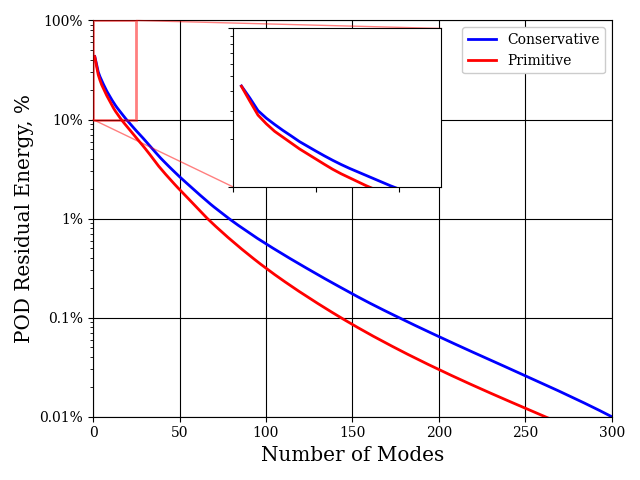
\includegraphics[width=0.8\linewidth]{Chapters/HPROMResults/Images/nineElem/nineElem_pod_energy.png}
	\caption{\label{fig:nineElemPODEnergy}POD residual energy decay for nine-element combustor conservative and primitive state datasets.}
\end{figure}

\begin{figure}
	\begin{minipage}{0.48\linewidth}
		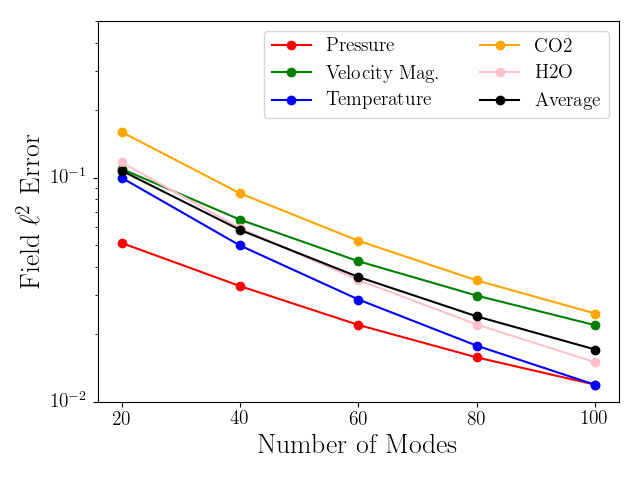
\includegraphics[width=0.99\linewidth,trim={0.5em 0.5em 0.5em 0.5em},clip]{Chapters/HPROMResults/Images/nineElem/projection_error_primitive.png}
		\caption{\label{fig:nineElemProjErrPrim}Primitive variables time-average projection error.}
	\end{minipage} \hspace{0.5em}
	\begin{minipage}{0.48\linewidth}
		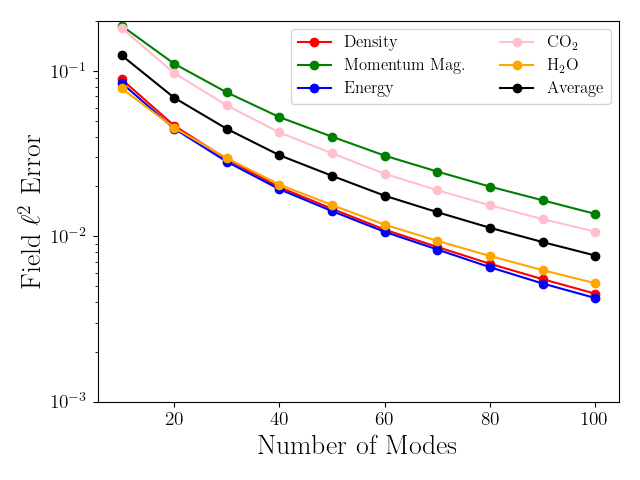
\includegraphics[width=0.99\linewidth,trim={0.5em 0.5em 0.5em 0.5em},clip]{Chapters/HPROMResults/Images/nineElem/projection_error_conservative.png}
		\caption{\label{fig:nineElemProjErrCons}Conservative variables time-average projection error.}
	\end{minipage}
\end{figure}

\subsection{Unsampled PROMs}

\begin{figure}
	\centering
	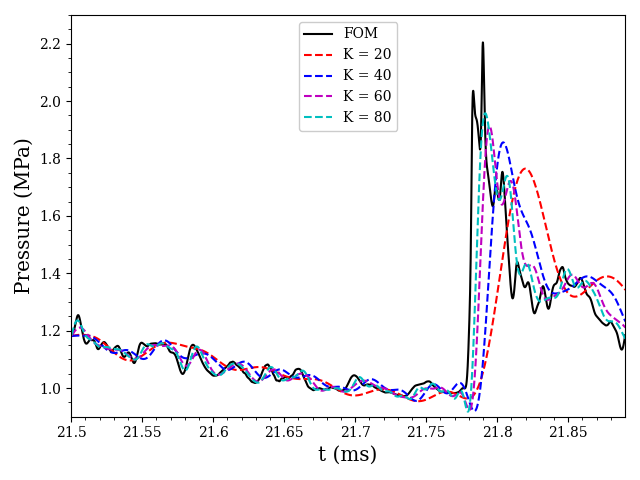
\includegraphics[width=0.6\linewidth]{Chapters/HPROMResults/Images/nineElem/unsampled/point_3_Static_Pressure.png}
	\caption{\label{fig:cvrcROMProbes}}
\end{figure}

\begin{figure}
	\begin{minipage}{0.45\linewidth}
		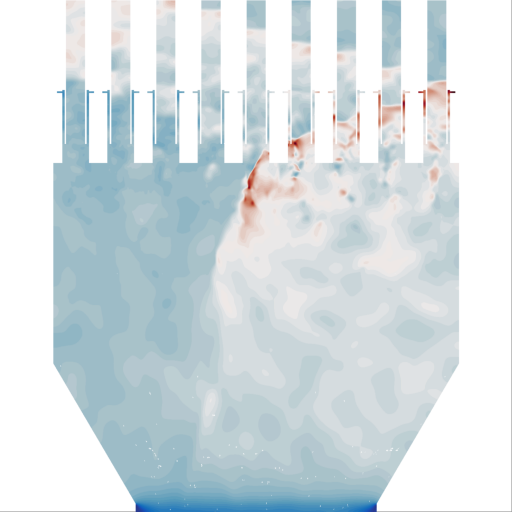
\includegraphics[width=0.99\linewidth,trim={0.5em 0.5em 0.5cm 0.5em},clip]{Chapters/HPROMResults/Images/nineElem/unsampled/fom/fig_z_Static_Pressure_218900.png}
	\end{minipage}
	\begin{minipage}{0.45\linewidth}
		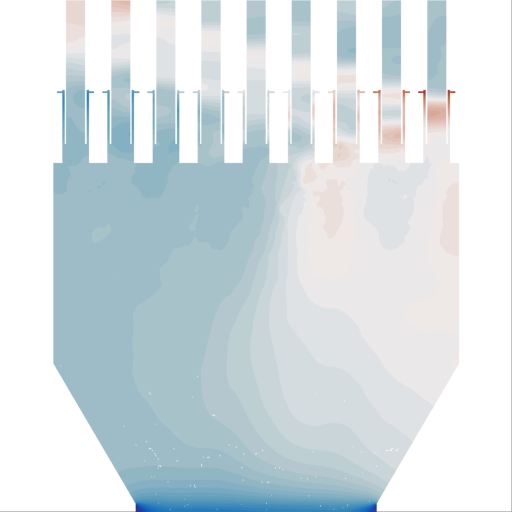
\includegraphics[width=0.99\linewidth,trim={0.5em 0.5em 0.5cm 0.5em},clip]{Chapters/HPROMResults/Images/nineElem/unsampled/k20/samp100p/UnsteadyFieldResults/Images/fig_z_Static_Pressure_4378.png}
	\end{minipage}

	\begin{minipage}{0.45\linewidth}
		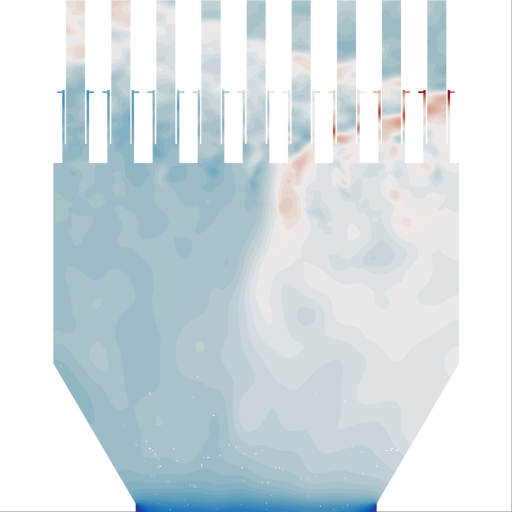
\includegraphics[width=0.99\linewidth,trim={0.5em 0.5em 0.5cm 0.5em},clip]{Chapters/HPROMResults/Images/nineElem/unsampled/k40/samp100p/UnsteadyFieldResults/Images/fig_z_Static_Pressure_4378.png}
	\end{minipage}
	\begin{minipage}{0.45\linewidth}
		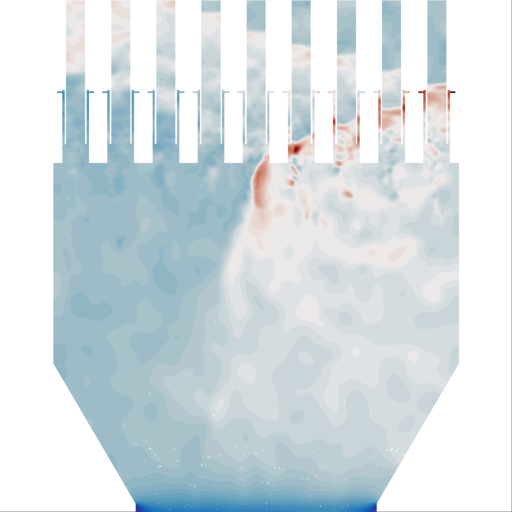
\includegraphics[width=0.99\linewidth,trim={0.5em 0.5em 0.5cm 0.5em},clip]{Chapters/HPROMResults/Images/nineElem/unsampled/k80/samp100p/UnsteadyFieldResults/Images/fig_z_Static_Pressure_4378.png}
	\end{minipage}
	\caption{\label{fig:cvrcROMPressureContours}Nine-element MP-LSVT PROM pressure contours, $\timeVar = 21.89$ms. FOM at top left, $\numPrimModes=20$ at top right, $\numPrimModes=40$ at bottom left, $\numPrimModes=80$ at bottom right.}
\end{figure}

\begin{figure}
	\begin{minipage}{0.45\linewidth}
		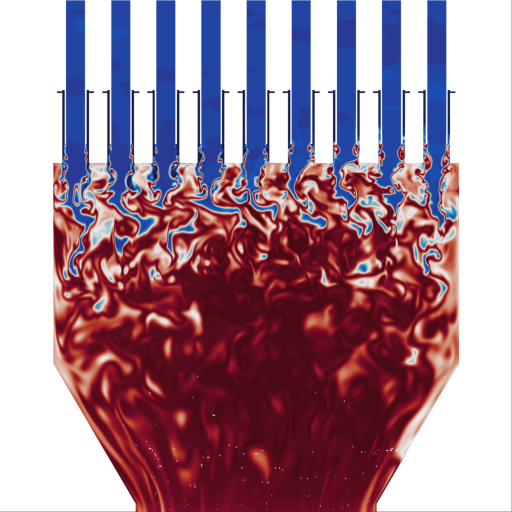
\includegraphics[width=0.99\linewidth,trim={0.5em 0.5em 0.5cm 0.5em},clip]{Chapters/HPROMResults/Images/nineElem/unsampled/fom/fig_z_Temperature_218900.png}
	\end{minipage}
	\begin{minipage}{0.45\linewidth}
		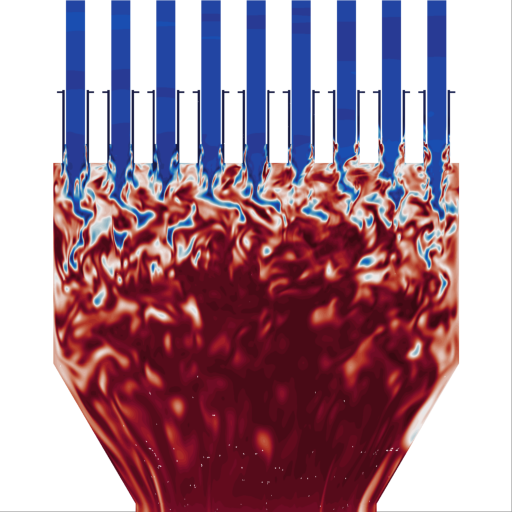
\includegraphics[width=0.99\linewidth,trim={0.5em 0.5em 0.5cm 0.5em},clip]{Chapters/HPROMResults/Images/nineElem/unsampled/k20/samp100p/UnsteadyFieldResults/Images/fig_z_Temperature_4378.png}
	\end{minipage}

	\begin{minipage}{0.45\linewidth}
		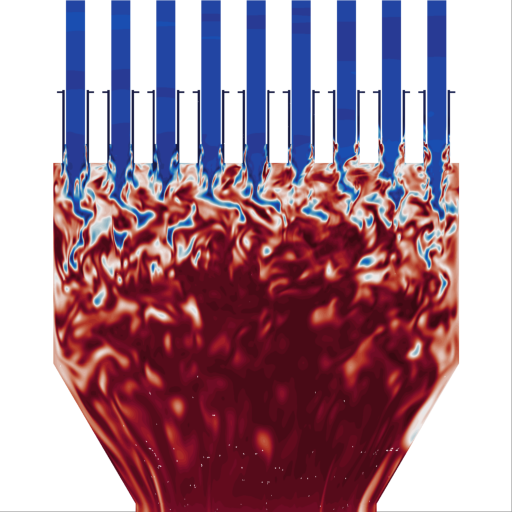
\includegraphics[width=0.99\linewidth,trim={0.5em 0.5em 0.5cm 0.5em},clip]{Chapters/HPROMResults/Images/nineElem/unsampled/k20/samp100p/UnsteadyFieldResults/Images/fig_z_Temperature_4378.png}
	\end{minipage}
	\begin{minipage}{0.45\linewidth}
		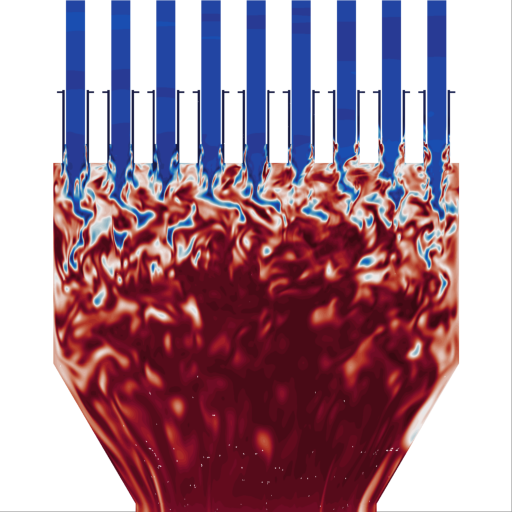
\includegraphics[width=0.99\linewidth,trim={0.5em 0.5em 0.5cm 0.5em},clip]{Chapters/HPROMResults/Images/nineElem/unsampled/k20/samp100p/UnsteadyFieldResults/Images/fig_z_Temperature_4378.png}
	\end{minipage}
	\caption{\label{fig:cvrcROMTempContours}Nine-element MP-LSVT PROM temperature contours, $\timeVar = 21.89$ms. FOM at top left, $\numPrimModes=20$ at top right, $\numPrimModes=40$ at bottom left, $\numPrimModes=80$ at bottom right.}
\end{figure}